\documentclass[11pt,a4paper]{article}
\usepackage{latexsym}
\usepackage{graphicx}
\usepackage{amssymb,amsmath}
\usepackage{mathtools,braket}
\usepackage[english]{babel}
\usepackage{caption}
\usepackage{subcaption}
\usepackage{graphicx}

% Parametri di stampa
\setlength{\topmargin}{-2.5cm} \setlength{\oddsidemargin}{0.3cm}
\setlength{\evensidemargin}{0.3cm}
%
\textheight=23.0truecm \textwidth=16.0truecm
%
\headheight=1.0cm \headsep=1.0cm
%
\renewcommand{\baselinestretch}{1.1}
\setlength{\unitlength}{1mm}

\parindent=6pt

%%%%%%%%%%%%%%%%%%%%%%%%%%%%%%%%%%%%%%%%%%%%%%%%%%%%%%%%%%%%%%%%%%%%%%%%%%%%

\newcommand{\be}{\begin{equation}}
\newcommand{\ee}{\end{equation}}
\newcommand{\bea}{\begin{eqnarray}}
\newcommand{\eea}{\end{eqnarray}}
\newcommand{\al}{\alpha}
\newcommand{\br}{\bar{\rho}}
\newcommand{\bg}{\bar{g}}
\newcommand{\bpi}{\bar{\pi}}

\newcommand{\op}[1]{\hat {#1}}

%%%%%%%%%%%%%%%%%%%%%%%%%%%%%%%%%%%%%%%%%%%%%%%%%%%%%%%%%%%%%%%%%%%%%%%%%%%%

\begin{document}

%%%%%%%%%%%%%%%%%%%%%%%%%%%%%%%%%%%%%%%%%%%%%%%%%%%%%%%%%%%%%%%%%%%%%%%%%%%%


\section*{Supplementary}

As stated in the main text we have investigated the effects of the size and dimension of a molecule in terms of the multi-threshold
structure of the excitation landscape. 
We may affirm that the number of localized excitations above the first ionization potential of the molecule typically grows with the
number of atoms of the molecule. This is simply due to the fact the bigger molecules behave as wider potential well and so the number of
(localized) empty KS states grows with the size....   


\begin{figure}[h]
    \centering
    \begin{subfigure}[t]{0.48\textwidth}
        \centering
        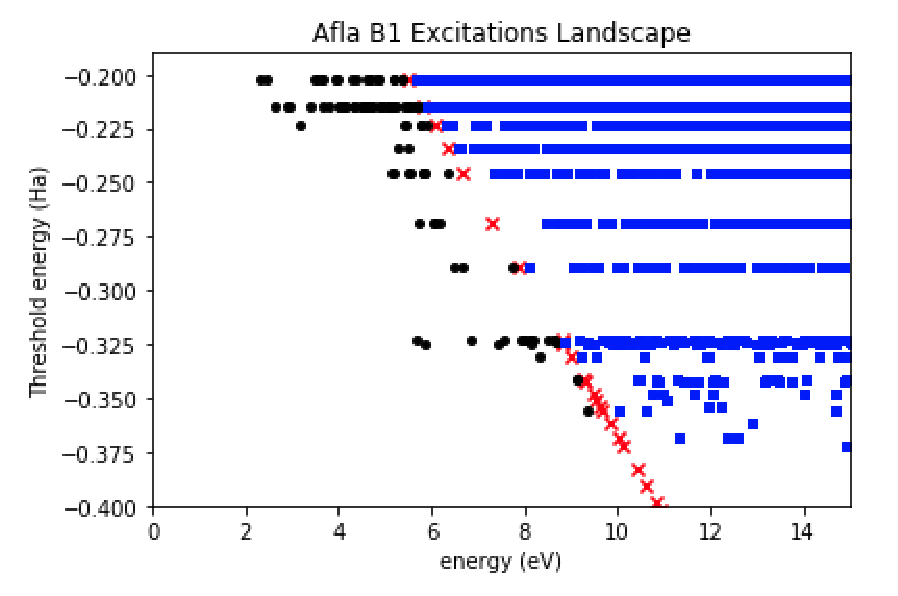
\includegraphics[width=\linewidth]{Aflatoxin_ExcitationLandscape.eps} 
        \caption{Aflatoxin} \label{fig:a}
    \end{subfigure}
    \hfill
    \begin{subfigure}[t]{0.48\textwidth}
        \centering
        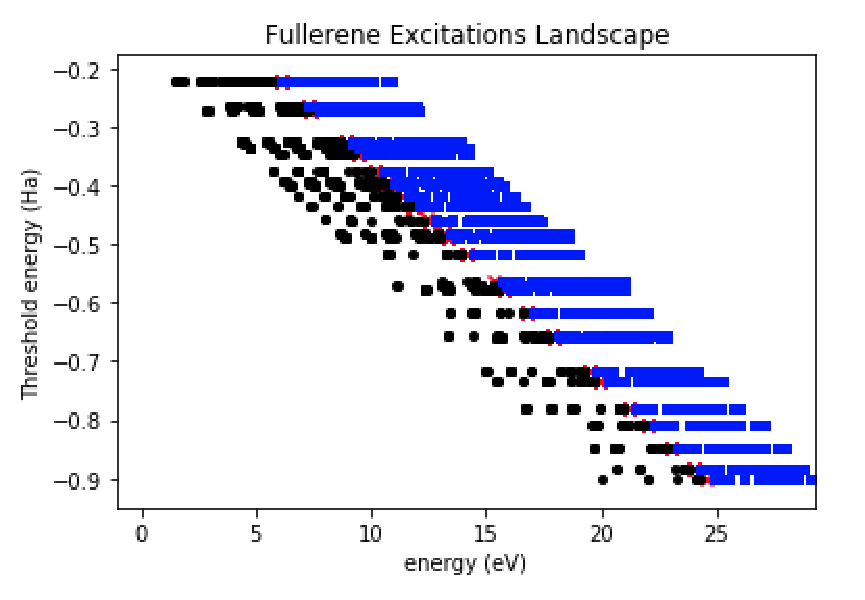
\includegraphics[width=\linewidth]{C60_ExcitationLandscape.eps} 
        \caption{$C_{60}$} \label{fig:b}
    \end{subfigure}

%     \vspace{1cm}
%     \begin{subfigure}[t]{\textwidth}
%     \centering
%         \includegraphics[width=\linewidth]{example-image-c.pdf} 
%         \caption{Price regulation} \label{fig:timing3}
%     \end{subfigure}
    \caption{Some general caption of all the figures....}
\end{figure}

%%%%%%%%%%%%%%%%%%%%%%%%%%%%%%%%%%%%%%%%%%%%%%%%%%%%%%%%%%%%%%%%%%%%%%%%%%%%

\end{document}

%%%%%%%%%%%%%%%%%%%%%%%%%%%%%%%%%%%%%%%%%%%%%%%%%%%%%%%%%%%%%%%%%%%%%%%%%%%%
